%
\section{Definizione di fluido}
Un fluido è un materiale che non è in grado di sopportare sforzi di taglio, quando è in quiete o in moto con velocità uniforme in un sistema di riferimento inerziale (invarianza galileiana).
I fluidi ``ordinari'' sono isotropi, cioè sono indipendenti dall'orientazione nello spazio.
Un fluido isotropo in quiete è quindi caratterizzato da uno stato di sforzo idrostatico,
\begin{equation}
 \mathbb{T}^{(s)} = - p \mathbb{I} \ ,
\end{equation}
avendo indicato con $\mathbb{T}^{(s)}$ il tensore degli sforzi in quiete, $p$ la pressione all'interno del fluido e $\mathbb{I}$ il tensore identità. Il vettore sforzo $\bm{t_n}$ \textit{agente su} una superficie di fluido con normale $\bm{\hat{n}}$ si ottiene tramite il \textbf{teorema di Cauchy} per i mezzi continui
\begin{equation}
 \bm{t_n} = \bm{\hat{n}} \cdot \mathbb{T} \ ,
\end{equation}
 che lega il vettore sforzo al tensore degli sforzi tramite il versore normale alla superficie considerata, e che nel caso di fluido in quiete, diventa
\begin{equation}
 \bm{t_n}^{(s)} = \bm{\hat{n}} \cdot \mathbb{T}^{(s)}  = - p \bm{\hat{n}} \ .
\end{equation} 
Per il principio di azione e reazione, lo sforzo agente su un materiale a contatto con un fluido è di intensità uguale e direzione opposta. La risultante $\bm{R}$ delle forze agenti su un volume di fluido $V$ è data dalla somma dell'integrale su $V$ delle forze di volume $\bm{f}$ e dell'integrale sulla superficie $S$, contorno del volume $V$, del vettore sforzo $\bm{t_n}$,
\begin{equation}
 \bm{R} = \int_V \bm{f} + \oint_S \bm{t_n} \ . 
\end{equation}

%
\section{Equazione di equilibrio: forma integrale e differenziale}
Un sistema meccanico è in equilibrio quando la risultante delle forze esterne e la risultante dei momenti esterni agenti sul fluido sono nulle,
\begin{equation}
\begin{cases}
 \bm{0} = \bm{R}^{ext} \\
 \bm{0} = \bm{M}^{ext}  \ .
\end{cases} 
\end{equation}
 Per un mezzo continuo non polare, è possibile dimostrare che l'equilibrio ai momenti si riduce alla condizione di simmetria del tensore degli sforzi.
L'equilibrio delle forze agenti su un volume di fluido $V$ in quiete, delimitato dalla superficie $\partial V = S$, soggetto a forze per unità di volume $\bm{f}$ in $V$ e forze per unità di superficie $\bm{t_n}=-p \bm{\hat{n}}$ su $S$ diventa
\begin{equation}
 \bm{0} = \bm{R}^{ext} = \int_V \bm{f} + \oint_S \bm{t_n} = \int_V \bm{f} - \oint_S p \bm{\hat{n}} \ .
\end{equation}
La condizione appena ottenuta è una \textbf{condizione di equilibrio integrale}, per l'intero volume fluido $V$. Se il campo di pressione $p$ è sufficientemente regolare, è possibile applicare il teorema del gradiente (\ref{thm:grad}) all'integrale di superficie e raccogliere i termini a destra dell'uguale sotto un unico integrale di volume $V$,
\begin{equation}
 \bm{0} = \int_V \left( \bm{f} - \bm{\nabla} p \right) \ .
\end{equation}
Poiché la condizione di equilibrio deve essere valida indipendentemente dal volume $V$ considerato, imponendo che l'integranda sia identicamente nulla, si ottiene l'\textbf{equazione di equilibrio in forma differenziale}
\begin{equation}\label{eqn:statica:diff}
 \bm{f}(\bm{r}) - \bm{\nabla} p (\bm{r}) = \bm{0} \ ,
\end{equation}
dove è stata esplicitata la dipendenza dei campi $\bm{f}$, $p$ dall coordinata spaziale $\bm{r}$. Nel caso in cui sia noto il campo di forze di volume $\bm{f}$ all'interno del dominio considerato, l'equazione differenziale alle derivate parziali (\ref{eqn:statica:diff}), con le opportune condizioni al contorno, permette di calcolare il campo di pressione $p(\bm{r})$. 

\section{Legge di Stevino}
La legge di Stevino descrive il campo di pressione come funzione della quota, nelle vicinanze della superficie terrestre. La legge di Stevino viene ricavata dall'integrazione dell'equilibrio in forma differenziale (\ref{eqn:statica:diff}), nel caso in cui le forze di volume siano dovute alla gravità $\bm{f}(\bm{r}) = \rho(\bm{r}) \bm{g}(\bm{r})$, avendo indicato con $\rho(\bm{r})$ la densità del fluido e con $\bm{g}$ il campo di accelerazione gravitazionale,
\begin{equation}\label{eqn:statica:diff:g}
    - \bm{\nabla} p(\bm{r}) + \rho(\bm{r}) \bm{g}(\bm{r}) = \bm{0} \ .
\end{equation}
Nell'ipotesi di essere sufficientemente vicino alla terra da poter considerare il campo vettoriale $\bm{g}$ uniforme e diretto verso il basso lungo la normale alla superficie terrestre, è possibile scrivere l'equazione precedente in un sistema di coordinate cartesiane. Orientando l'asse $z$ verso l'alto lungo la normale alla superficie, le tre componenti cartesiane dell'equazione vettoriale sono
\begin{equation}
\begin{cases}
 \partial p(x,y,z) / \partial x = 0 \\
 \partial p(x,y,z) / \partial y = 0 \\ 
 \partial p(x,y,z) / \partial z = - \rho(x,y,z) g \ .
\end{cases}
\end{equation}
Dalle prime due equazioni si ricava che il campo di pressione non può dipendere dalle coordinate $x$, $y$ ed è quindi solo funzione di $z$. Poiché il campo di pressione dipende solo da $z$, $p = P(z)$, la terza equazione diventa un'equazione differenziale ordinaria,
\begin{equation}\label{eqn:statica:Pz}
  \dfrac{d P}{d z} = -\rho(x,y,z) g \ ,
\end{equation}
alla quale deve essere aggiunta una condizione al contorno del tipo $P(z_0) = p_0$.\footnote{In generale, servono delle condizioni di compabibilità dei dati affinché il problema sia risolvibile. Ad esempio, non dovrebbe essere difficile convincersi che il campo di densità deve dipendere solo dalla coordinata $z$ nel caso considerato.}
Senza ulteriori ipotesi, il problema composto dall'equazione (\ref{eqn:statica:Pz}) e dalla condizione al contorno necessaria ha come incognite il campo di pressione $P$ e il campo di densità $\rho$. 
In generale, per risolvere il problema è necessario la legge di stato del fluido che mette in relazione i due campi.
%
\newline \noindent
Nell'ipotesi che la densità $\rho$ e la forza di gravità siano costanti, la soluzione del problema (\ref{eqn:statica:Pz}) coincide con la \textit{legge di Stevino},
\begin{equation}
 p(z) + \rho g z = p_0 = \text{cost} \ ,
\end{equation}
avendo orientato l'asse $z$ verso l'alto e imposto la condizione al contorno in $z_0 = 0$.
% Nel caso in cui la densità non sia costante, ma che dipenda dallo stato termodinamico, per risolvere il problema è necessaria l'equazione di stato del fluido.
\begin{exercise}\label{exe:stdatm:cart}
    Utilizzando la legge di stato dei gas perfetti per l'aria, $P = \rho R T$, e l'approssimazione lineare dell'andamento della temperatura con la quota $z$, con gradiente termico $dT/dz=a=-6.5\degree/km$, si ricavi l'andamento con la quota $z$ delle variabili termodinamiche $(P,\rho, T)$ per l'atrmosfera standard. Si trascuri l'andamento di $g$ con la quota. Trascurando la curvatura terrestre, si utilizzi un sistema di coordinate cartesiane per scrivere le componenti dell'equazione vettoriale (\ref{eqn:statica:diff:g}).
\end{exercise}
\begin{exercise}\label{exe:stdatm:sphe}
    Utilizzando la legge di stato dei gas perfetti per l'aria, $P = \rho R T$, e l'approssimazione lineare dell'andamento della temperatura con la quota $r$, con gradiente termico $dT/dr=a=-6.5\degree/km$, si ricavi l'andamento con la quota $r$ delle variabili termodinamiche $(P,\rho, T)$ per l'atrmosfera standard, senza trascurare l'effetto della curvatura terrestre. Si utilizzi un sistema di coordinate sferiche per scrivere le componenti dell'equazione vettoriale (\ref{eqn:statica:diff:g}). Si valuti poi l'errore che si commette nell'esercizio \ref{exe:stdatm:cart} trascurando la curvatura terrestre sul calcolo delle variabili termodinamiche a quota $z = 10 \ km$.
\end{exercise}
%
\section{Galleggiamento di un corpo immerso in un fluido}
Un corpo immerso in fluido riceve dal basso verso l'alto una spinta uguale al peso della massa del fluido spostato. Se un corpo di volume $V_s$ immerso in un fluido $\rho_f$ ne sposta un volume $\tilde{V}_f$, su di esso agisce una forza (di Archimede o di galleggiamento)
\begin{equation}
    \bm{F}_{Arch} = - \rho_f \tilde{V}_f \bm{g} = - \int_{\tilde{V}_f} \rho_f \bm{g} \ .
\end{equation}
La legge di Archimede vale per un sistema immerso nel campo di gravità $\bm{g}$, uniforme in spazio.
\newline \noindent
Forze di galleggimento nascono su un corpo immerso in un fluido in cui c'è un gradiente di pressione. La legge di Archimede è solo un caso particolare di galleggiamento, forse il più evidente, per il quale il campo di gravità è all'origine del gradiente di pressione. In generale, la forza di galleggiamento su un corpo immerso completamente in un fluido vale
\begin{equation}
    \bm{F}_{gall} = -\int_{S_s} p \bm{\hat{n}} = - \int_{V_s} \bm{\nabla} p \ .
\end{equation}
Un esempio di galleggiamento di interesse aeronautico si incontra quando si svolge un esperimento in galleria del vento, se nella camera di prova è presente un gradiente di pressione diretto nella direzione $\bm{\hat{x}}$ della corrente. Se in prima approssimazione si considera un gradiente di pressione $\bm{\nabla}p = - G_P \bm{\hat{x}}$, $G_P>0$ e costante, si può stimare la forza di galleggiamento $\bm{F}_{gall} = V_s G_P \bm{\hat{x}}$ dovuta al gradiente di pressione in galleria del vento, assente in condizioni di aria libera. Questa azione contribuisce al valore misurato della resistenza del modello.
%
La valutazione di questa azione ``spuria'' sul corpo e la correzione delle misure effettuate rientrano nell'ambito delle \textit{correzioni di galleria}.

% \vspace{3cm}


% \section{Risultante e punto di applicazione delle forze di galleggiamento: equilibrio e stabilità di corpi galleggianti}

\vspace{10pt}
Si ritorna ora sulla legge di Archimede che descrive le forza di galleggiamento che un fluido esercita su un corpo immerso. Nel problema di un corpo immerso in un fluido, la risultante delle forze di galleggiamento entra nell'equazione di equilibrio del corpo in direzione verticale (direzione della gravità, \textbf{g}). Il punto di applicazione della risultante delle forze di galleggiamento e la sua posizione relativa rispetto al baricentro del corpo influenzano la stabilità delle condizioni di equilibrio.

\subsection{Risultante delle forze: legge di Archimede}
%
\begin{figure}[t]
 \centering
 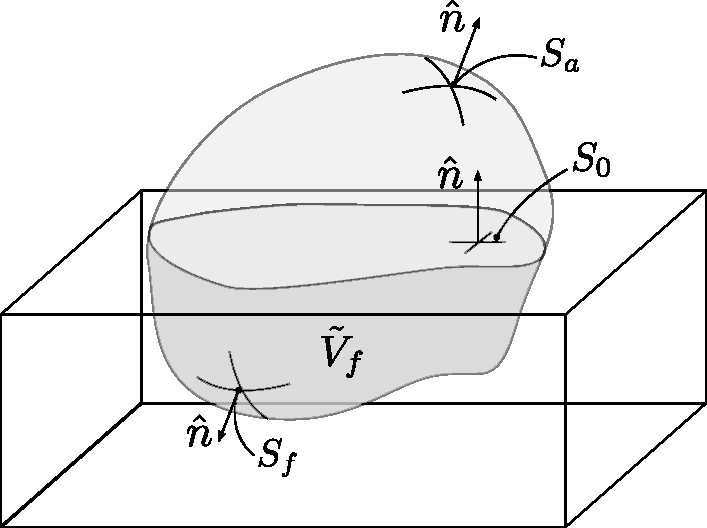
\includegraphics[width=0.5\textwidth]{./fig/archimede_01}
 \caption{Suddivisione delle superfici e dei volumi per la dimostrazione della legge di Archimede.}\label{fig:archimede_01}
\end{figure}
%
Si considera il problema di un corpo immerso in un fluido di densità uniforme $\rho$ molto maggiore della densità dell'aria: la pressione agente sulla superficie del corpo esposta all'aria si può considerare costante, uguale a $p_a$.
La legge di Stevino descrive la distribuzione di pressione all'interno del fluido. Si sceglie l'asse $z$ in direzione verticale, così che il campo di gravità è $\bm{g} = -g \bm{\hat{z}}$. Scegliendo l'origine dell'asse $z$ in corrispondenza del pelo libero, la pressione all'interno del fluido vale $p(z) = p_a - \rho g z$, per $z < 0$. Facendo riferimento alla figura \ref{fig:archimede_01}, si può calcolare la risultante delle forze $\bm{R}$ come
\begin{equation}
\begin{aligned}
    \bm{R} & = - \oint_{S} p \bm{\hat{n}} = 
               - \int_{S_a} p \bm{\hat{n}} - \int_{S_f} p \bm{\hat{n}} = \\
        & =    - \int_{S_a} p_a \bm{\hat{n}} - \int_{S_f} p_a \bm{\hat{n}} + 
                 \int_{S_f} \rho g z \bm{\hat{n}} = \\
        & =    - \underbrace{\int_{S} p_a \bm{\hat{n}}}_{=0} + 
                 \int_{S_f} \rho g z \bm{\hat{n}} = \\
        & =      \int_{S_f} \rho g z \bm{\hat{n}} + 
                 \underbrace{\int_{S_0} \rho g z \bm{\hat{n}}}_{=0, \ z|_{S_0} = 0} =
                 \oint_{\tilde{S}_f} \rho g z \bm{\hat{n}} = 
                 \int_{\tilde{V}_f} \rho g \bm{\hat{z} } = 
                 \rho \tilde{V}_f g \bm{\hat{z}} = 
                 M_{\tilde{V}_f} g \bm{\hat{z}} \ ,
\end{aligned}
\end{equation}
avendo sommato l'integrale nullo $\int_{S_0} \rho g z \bm{\hat{n}}$, per poter ottenere l'integrale di $\rho g z$ sulla superficie $\tilde{S}_f = S_f \cup S_0$ e applicare il teorema del gradiente (\ref{thm:grad}).
Come stabilito dal principio di Archimede, la risultante delle forze di galleggiamento $\bm{R}$ agenti sul corpo agisce dal basso verso l'alto con un'intensità pari al peso del volume di fluido spostato, $M_{\tilde{V}_f} g$.

\subsection{Punto di applicazione}
Il punto di applicazione della forza di galleggiamento è il punto dove bisogna applicare la risultante delle forze per ottenere un sistema di azioni equivalente al sistema di azioni continuo generato dalla pressione.
Dall'equivalenza ai momenti dei due sistemi di azioni, si ottiene
\begin{equation}
\begin{aligned}
\bm{r}_O \times \bm{R} & = - \oint_{S} p \bm{r} \times \bm{\hat{n}} = 
    - \int_{S_a} p \bm{r} \times \bm{\hat{n}}
    - \int_{S_f} p \bm{r} \times \bm{\hat{n}} = \\
& = - \int_{S_a} p_a \bm{r} \times \bm{\hat{n}}
    - \int_{S_f} p_a \bm{r} \times \bm{\hat{n}} 
    + \int_{S_f} \rho g z \bm{r} \times \bm{\hat{n}} = \\
& = - \underbrace{\int_{S} p_a \bm{r} \times \bm{\hat{n}}}_{=0} + 
      \int_{S_f} \rho g z \bm{r} \times \bm{\hat{n}} = \\
& =   \int_{S_f} \rho g z \bm{r} \times \bm{\hat{n}} + 
      \underbrace{\int_{S_0} \rho g z \bm{r} \times \bm{\hat{n}}}_{=0, \ z|_{S_0} = 0} =\\
& =  \oint_{\tilde{S}_f} \rho g z \bm{r} \times \bm{\hat{n}} = 
     \oint_{\tilde{S}_f} \rho g \delta_{\ell z} r_{\ell} \epsilon_{ijk} r_j n_k = 
     \rho g \int_{\tilde{V}_f} \dfrac{\partial}{\partial r_k}( \delta_{\ell z} r_{\ell} \epsilon_{ijk} r_j ) = \\
    & = \rho g \int_{\tilde{V}_f} \delta_{\ell z} \epsilon_{ijk}\left(  \dfrac{\partial r_{\ell}}{\partial r_k} r_j + r_{\ell} \dfrac{\partial r_j}{\partial r_k} \right) = \\ 
    & = \rho g \int_{\tilde{V}_f} \delta_{\ell z} \epsilon_{ijk}\left( \delta_{\ell k}r_j + r_{\ell} \delta_{jk} \right) = \\
    & = \rho g \int_{\tilde{V}_f} \epsilon_{ijz} r_j + \delta_{\ell z} \underbrace{\epsilon_{ijj}}_{ = 0} r_{\ell} = \\
    & = \rho g \int_{\tilde{V}_f}  \bm{r} \times \bm{\hat{z}} \ .
\end{aligned}
\end{equation}
Usando un sistema di assi catesiani e ricordando che $\bm{R} = R \bm{\hat{z}}$, si può scomprre l'equazione nelle componenti non nulle, $x$ e $y$, 
\begin{equation}
\begin{cases}
   x_0 R = \rho g \displaystyle\int_{\tilde{V}_f} x \\ \\
   y_0 R = \rho g \displaystyle\int_{\tilde{V}_f} y 
\end{cases} \qquad \rightarrow \qquad
\begin{cases}
    x_0 = \dfrac{\rho g}{R}  \displaystyle\int_{\tilde{V}_f} x  
        = \dfrac{1}{\tilde{V}_f}  \displaystyle\int_{\tilde{V}_f} x 
    \\ \\
    y_0 = \dfrac{\rho g}{R}  \displaystyle\int_{\tilde{V}_f} y 
        = \dfrac{1}{\tilde{V}_f}  \displaystyle\int_{\tilde{V}_f} y \ .
\end{cases}
\end{equation}


\subsection{Stabilità statica dell'equilibrio}


% \section{}




